\documentclass[1p]{elsarticle_modified}
%\bibliographystyle{elsarticle-num}

%\usepackage[colorlinks]{hyperref}
%\usepackage{abbrmath_seonhwa} %\Abb, \Ascr, \Acal ,\Abf, \Afrak
\usepackage{amsfonts}
\usepackage{amssymb}
\usepackage{amsmath}
\usepackage{amsthm}
\usepackage{scalefnt}
\usepackage{amsbsy}
\usepackage{kotex}
\usepackage{caption}
\usepackage{subfig}
\usepackage{color}
\usepackage{graphicx}
\usepackage{xcolor} %% white, black, red, green, blue, cyan, magenta, yellow
\usepackage{float}
\usepackage{setspace}
\usepackage{hyperref}

\usepackage{tikz}
\usetikzlibrary{arrows}

\usepackage{multirow}
\usepackage{array} % fixed length table
\usepackage{hhline}

%%%%%%%%%%%%%%%%%%%%%
\makeatletter
\renewcommand*\env@matrix[1][\arraystretch]{%
	\edef\arraystretch{#1}%
	\hskip -\arraycolsep
	\let\@ifnextchar\new@ifnextchar
	\array{*\c@MaxMatrixCols c}}
\makeatother %https://tex.stackexchange.com/questions/14071/how-can-i-increase-the-line-spacing-in-a-matrix
%%%%%%%%%%%%%%%

\usepackage[normalem]{ulem}

\newcommand{\msout}[1]{\ifmmode\text{\sout{\ensuremath{#1}}}\else\sout{#1}\fi}
%SOURCE: \msout is \stkout macro in https://tex.stackexchange.com/questions/20609/strikeout-in-math-mode

\newcommand{\cancel}[1]{
	\ifmmode
	{\color{red}\msout{#1}}
	\else
	{\color{red}\sout{#1}}
	\fi
}

\newcommand{\add}[1]{
	{\color{blue}\uwave{#1}}
}

\newcommand{\replace}[2]{
	\ifmmode
	{\color{red}\msout{#1}}{\color{blue}\uwave{#2}}
	\else
	{\color{red}\sout{#1}}{\color{blue}\uwave{#2}}
	\fi
}

\newcommand{\Sol}{\mathcal{S}} %segment
\newcommand{\D}{D} %diagram
\newcommand{\A}{\mathcal{A}} %arc


%%%%%%%%%%%%%%%%%%%%%%%%%%%%%5 test

\def\sl{\operatorname{\textup{SL}}(2,\Cbb)}
\def\psl{\operatorname{\textup{PSL}}(2,\Cbb)}
\def\quan{\mkern 1mu \triangleright \mkern 1mu}

\theoremstyle{definition}
\newtheorem{thm}{Theorem}[section]
\newtheorem{prop}[thm]{Proposition}
\newtheorem{lem}[thm]{Lemma}
\newtheorem{ques}[thm]{Question}
\newtheorem{cor}[thm]{Corollary}
\newtheorem{defn}[thm]{Definition}
\newtheorem{exam}[thm]{Example}
\newtheorem{rmk}[thm]{Remark}
\newtheorem{alg}[thm]{Algorithm}

\newcommand{\I}{\sqrt{-1}}
\begin{document}

%\begin{frontmatter}
%
%\title{Boundary parabolic representations of knots up to 8 crossings}
%
%%% Group authors per affiliation:
%\author{Yunhi Cho} 
%\address{Department of Mathematics, University of Seoul, Seoul, Korea}
%\ead{yhcho@uos.ac.kr}
%
%
%\author{Seonhwa Kim} %\fnref{s_kim}}
%\address{Center for Geometry and Physics, Institute for Basic Science, Pohang, 37673, Korea}
%\ead{ryeona17@ibs.re.kr}
%
%\author{Hyuk Kim}
%\address{Department of Mathematical Sciences, Seoul National University, Seoul 08826, Korea}
%\ead{hyukkim@snu.ac.kr}
%
%\author{Seokbeom Yoon}
%\address{Department of Mathematical Sciences, Seoul National University, Seoul, 08826,  Korea}
%\ead{sbyoon15@snu.ac.kr}
%
%\begin{abstract}
%We find all boundary parabolic representation of knots up to 8 crossings.
%
%\end{abstract}
%\begin{keyword}
%    \MSC[2010] 57M25 
%\end{keyword}
%
%\end{frontmatter}

%\linenumbers
%\tableofcontents
%
\newcommand\colored[1]{\textcolor{white}{\rule[-0.35ex]{0.8em}{1.4ex}}\kern-0.8em\color{red} #1}%
%\newcommand\colored[1]{\textcolor{white}{ #1}\kern-2.17ex	\textcolor{white}{ #1}\kern-1.81ex	\textcolor{white}{ #1}\kern-2.15ex\color{red}#1	}

{\Large $\underline{12a_{0598}~(K12a_{0598})}$}

\setlength{\tabcolsep}{10pt}
\renewcommand{\arraystretch}{1.6}
\vspace{1cm}\begin{tabular}{m{100pt}>{\centering\arraybackslash}m{274pt}}
\multirow{5}{120pt}{
	\centering
	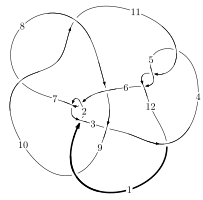
\includegraphics[width=112pt]{../../../GIT/diagram.site/Diagrams/png/1399_12a_0598.png}\\
\ \ \ A knot diagram\footnotemark}&
\allowdisplaybreaks
\textbf{Linearized knot diagam} \\
\cline{2-2}
 &
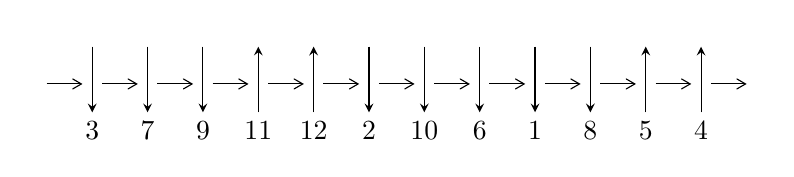
\begin{tikzpicture}[x=20pt, y=17pt]
	% nodes
	\node (C0) at (0, 0) {};
	\node (C1) at (1, 0) {};
	\node (C1U) at (1, +1) {};
	\node (C1D) at (1, -1) {3};

	\node (C2) at (2, 0) {};
	\node (C2U) at (2, +1) {};
	\node (C2D) at (2, -1) {7};

	\node (C3) at (3, 0) {};
	\node (C3U) at (3, +1) {};
	\node (C3D) at (3, -1) {9};

	\node (C4) at (4, 0) {};
	\node (C4U) at (4, +1) {};
	\node (C4D) at (4, -1) {11};

	\node (C5) at (5, 0) {};
	\node (C5U) at (5, +1) {};
	\node (C5D) at (5, -1) {12};

	\node (C6) at (6, 0) {};
	\node (C6U) at (6, +1) {};
	\node (C6D) at (6, -1) {2};

	\node (C7) at (7, 0) {};
	\node (C7U) at (7, +1) {};
	\node (C7D) at (7, -1) {10};

	\node (C8) at (8, 0) {};
	\node (C8U) at (8, +1) {};
	\node (C8D) at (8, -1) {6};

	\node (C9) at (9, 0) {};
	\node (C9U) at (9, +1) {};
	\node (C9D) at (9, -1) {1};

	\node (C10) at (10, 0) {};
	\node (C10U) at (10, +1) {};
	\node (C10D) at (10, -1) {8};

	\node (C11) at (11, 0) {};
	\node (C11U) at (11, +1) {};
	\node (C11D) at (11, -1) {5};

	\node (C12) at (12, 0) {};
	\node (C12U) at (12, +1) {};
	\node (C12D) at (12, -1) {4};
	\node (C13) at (13, 0) {};

	% arrows
	\draw[->,>={angle 60}]
	(C0) edge (C1) (C1) edge (C2) (C2) edge (C3) (C3) edge (C4) (C4) edge (C5) (C5) edge (C6) (C6) edge (C7) (C7) edge (C8) (C8) edge (C9) (C9) edge (C10) (C10) edge (C11) (C11) edge (C12) (C12) edge (C13) ;	\draw[->,>=stealth]
	(C1U) edge (C1D) (C2U) edge (C2D) (C3U) edge (C3D) (C4D) edge (C4U) (C5D) edge (C5U) (C6U) edge (C6D) (C7U) edge (C7D) (C8U) edge (C8D) (C9U) edge (C9D) (C10U) edge (C10D) (C11D) edge (C11U) (C12D) edge (C12U) ;
	\end{tikzpicture} \\
\hhline{~~} \\& 
\textbf{Solving Sequence} \\ \cline{2-2} 
 &
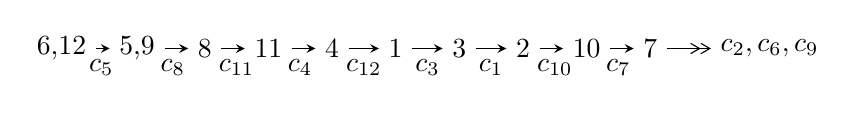
\begin{tikzpicture}[x=23pt, y=7pt]
	% node
	\node (A0) at (-1/8, 0) {6,12};
	\node (A1) at (17/16, 0) {5,9};
	\node (A2) at (17/8, 0) {8};
	\node (A3) at (25/8, 0) {11};
	\node (A4) at (33/8, 0) {4};
	\node (A5) at (41/8, 0) {1};
	\node (A6) at (49/8, 0) {3};
	\node (A7) at (57/8, 0) {2};
	\node (A8) at (65/8, 0) {10};
	\node (A9) at (73/8, 0) {7};
	\node (C1) at (1/2, -1) {$c_{5}$};
	\node (C2) at (13/8, -1) {$c_{8}$};
	\node (C3) at (21/8, -1) {$c_{11}$};
	\node (C4) at (29/8, -1) {$c_{4}$};
	\node (C5) at (37/8, -1) {$c_{12}$};
	\node (C6) at (45/8, -1) {$c_{3}$};
	\node (C7) at (53/8, -1) {$c_{1}$};
	\node (C8) at (61/8, -1) {$c_{10}$};
	\node (C9) at (69/8, -1) {$c_{7}$};
	\node (A10) at (11, 0) {$c_{2},c_{6},c_{9}$};

	% edge
	\draw[->,>=stealth]	
	(A0) edge (A1) (A1) edge (A2) (A2) edge (A3) (A3) edge (A4) (A4) edge (A5) (A5) edge (A6) (A6) edge (A7) (A7) edge (A8) (A8) edge (A9) ;
	\draw[->>,>={angle 60}]	
	(A9) edge (A10);
\end{tikzpicture} \\ 

\end{tabular} \\

\footnotetext{
The image of knot diagram is generated by the software ``\textbf{Draw programme}" developed by Andrew Bartholomew(\url{http://www.layer8.co.uk/maths/draw/index.htm\#Running-draw}), where we modified some parts for our purpose(\url{https://github.com/CATsTAILs/LinksPainter}).
}\phantom \\ \newline 
\centering \textbf{Ideals for irreducible components\footnotemark of $X_{\text{par}}$} 
 
\begin{align*}
I^u_{1}&=\langle 
-2.88484\times10^{108} u^{104}-5.09336\times10^{110} u^{103}+\cdots+8.35512\times10^{110} b-2.14019\times10^{110},\\
\phantom{I^u_{1}}&\phantom{= \langle  }6.52267\times10^{110} u^{104}+1.42528\times10^{111} u^{103}+\cdots+8.35512\times10^{110} a-2.67566\times10^{111},\;u^{105}+3 u^{104}+\cdots+3 u-1\rangle \\
\\
\end{align*}
\raggedright * 1 irreducible components of $\dim_{\mathbb{C}}=0$, with total 105 representations.\\
\footnotetext{All coefficients of polynomials are rational numbers. But the coefficients are sometimes approximated in decimal forms when there is not enough margin.}
\newpage
\renewcommand{\arraystretch}{1}
\centering \section*{I. $I^u_{1}= \langle -2.88\times10^{108} u^{104}-5.09\times10^{110} u^{103}+\cdots+8.36\times10^{110} b-2.14\times10^{110},\;6.52\times10^{110} u^{104}+1.43\times10^{111} u^{103}+\cdots+8.36\times10^{110} a-2.68\times10^{111},\;u^{105}+3 u^{104}+\cdots+3 u-1 \rangle$}
\flushleft \textbf{(i) Arc colorings}\\
\begin{tabular}{m{7pt} m{180pt} m{7pt} m{180pt} }
\flushright $a_{6}=$&$\begin{pmatrix}1\\0\end{pmatrix}$ \\
\flushright $a_{12}=$&$\begin{pmatrix}0\\u\end{pmatrix}$ \\
\flushright $a_{5}=$&$\begin{pmatrix}1\\u^2\end{pmatrix}$ \\
\flushright $a_{9}=$&$\begin{pmatrix}-0.780679 u^{104}-1.70588 u^{103}+\cdots-4.20124 u+3.20242\\0.00345278 u^{104}+0.609609 u^{103}+\cdots+0.427791 u+0.256153\end{pmatrix}$ \\
\flushright $a_{8}=$&$\begin{pmatrix}-0.777226 u^{104}-1.09627 u^{103}+\cdots-3.77344 u+3.45857\\0.00345278 u^{104}+0.609609 u^{103}+\cdots+0.427791 u+0.256153\end{pmatrix}$ \\
\flushright $a_{11}=$&$\begin{pmatrix}- u\\- u^3+u\end{pmatrix}$ \\
\flushright $a_{4}=$&$\begin{pmatrix}- u^2+1\\- u^4+2 u^2\end{pmatrix}$ \\
\flushright $a_{1}=$&$\begin{pmatrix}u^5-2 u^3+u\\u^7-3 u^5+2 u^3+u\end{pmatrix}$ \\
\flushright $a_{3}=$&$\begin{pmatrix}0.00955622 u^{104}-0.543671 u^{103}+\cdots+1.65157 u-0.986304\\0.0176604 u^{104}+0.542716 u^{103}+\cdots-0.341063 u-0.0571853\end{pmatrix}$ \\
\flushright $a_{2}=$&$\begin{pmatrix}0.455592 u^{104}+1.26266 u^{103}+\cdots-2.33857 u+0.208499\\-0.376670 u^{104}-1.24789 u^{103}+\cdots+2.98305 u-0.410701\end{pmatrix}$ \\
\flushright $a_{10}=$&$\begin{pmatrix}-0.591260 u^{104}-0.829214 u^{103}+\cdots-5.61982 u+3.23227\\0.261471 u^{104}+1.08908 u^{103}+\cdots+1.38898 u+0.232872\end{pmatrix}$ \\
\flushright $a_{7}=$&$\begin{pmatrix}-0.362637 u^{104}-0.610684 u^{103}+\cdots+3.25250 u+0.271811\\-0.447610 u^{104}-0.767496 u^{103}+\cdots-1.00923 u+0.0171223\end{pmatrix}$\\&\end{tabular}
\flushleft \textbf{(ii) Obstruction class $= -1$}\\~\\
\flushleft \textbf{(iii) Cusp Shapes $= -7.93747 u^{104}-23.0087 u^{103}+\cdots+20.0215 u-13.3715$}\\~\\
\newpage\renewcommand{\arraystretch}{1}
\flushleft \textbf{(iv) u-Polynomials at the component}\newline \\
\begin{tabular}{m{50pt}|m{274pt}}
Crossings & \hspace{64pt}u-Polynomials at each crossing \\
\hline $$\begin{aligned}c_{1}\end{aligned}$$&$\begin{aligned}
&u^{105}+45 u^{104}+\cdots+13 u+1
\end{aligned}$\\
\hline $$\begin{aligned}c_{2},c_{6}\end{aligned}$$&$\begin{aligned}
&u^{105}-3 u^{104}+\cdots+u+1
\end{aligned}$\\
\hline $$\begin{aligned}c_{3}\end{aligned}$$&$\begin{aligned}
&u^{105}- u^{104}+\cdots-23 u+1
\end{aligned}$\\
\hline $$\begin{aligned}c_{4},c_{5},c_{11}\end{aligned}$$&$\begin{aligned}
&u^{105}-3 u^{104}+\cdots+3 u+1
\end{aligned}$\\
\hline $$\begin{aligned}c_{7},c_{10}\end{aligned}$$&$\begin{aligned}
&u^{105}- u^{104}+\cdots- u+1
\end{aligned}$\\
\hline $$\begin{aligned}c_{8}\end{aligned}$$&$\begin{aligned}
&u^{105}-3 u^{104}+\cdots-119583 u+5771
\end{aligned}$\\
\hline $$\begin{aligned}c_{9}\end{aligned}$$&$\begin{aligned}
&u^{105}+47 u^{104}+\cdots+6197 u+361
\end{aligned}$\\
\hline $$\begin{aligned}c_{12}\end{aligned}$$&$\begin{aligned}
&u^{105}+9 u^{104}+\cdots+4875 u+725
\end{aligned}$\\
\hline
\end{tabular}\\~\\
\newpage\renewcommand{\arraystretch}{1}
\flushleft \textbf{(v) Riley Polynomials at the component}\newline \\
\begin{tabular}{m{50pt}|m{274pt}}
Crossings & \hspace{64pt}Riley Polynomials at each crossing \\
\hline $$\begin{aligned}c_{1}\end{aligned}$$&$\begin{aligned}
&y^{105}+31 y^{104}+\cdots+29 y-1
\end{aligned}$\\
\hline $$\begin{aligned}c_{2},c_{6}\end{aligned}$$&$\begin{aligned}
&y^{105}-45 y^{104}+\cdots+13 y-1
\end{aligned}$\\
\hline $$\begin{aligned}c_{3}\end{aligned}$$&$\begin{aligned}
&y^{105}+3 y^{104}+\cdots+65 y-1
\end{aligned}$\\
\hline $$\begin{aligned}c_{4},c_{5},c_{11}\end{aligned}$$&$\begin{aligned}
&y^{105}-89 y^{104}+\cdots+13 y-1
\end{aligned}$\\
\hline $$\begin{aligned}c_{7},c_{10}\end{aligned}$$&$\begin{aligned}
&y^{105}-69 y^{104}+\cdots-303 y-1
\end{aligned}$\\
\hline $$\begin{aligned}c_{8}\end{aligned}$$&$\begin{aligned}
&y^{105}+603 y^{104}+\cdots-4958310211 y-33304441
\end{aligned}$\\
\hline $$\begin{aligned}c_{9}\end{aligned}$$&$\begin{aligned}
&y^{105}-601 y^{104}+\cdots+13093821 y-130321
\end{aligned}$\\
\hline $$\begin{aligned}c_{12}\end{aligned}$$&$\begin{aligned}
&y^{105}+43 y^{104}+\cdots+17234825 y-525625
\end{aligned}$\\
\hline
\end{tabular}\\~\\
\newpage\flushleft \textbf{(vi) Complex Volumes and Cusp Shapes}
$$\begin{array}{c|c|c}  
\text{Solutions to }I^u_{1}& \I (\text{vol} + \sqrt{-1}CS) & \text{Cusp shape}\\
 \hline 
\begin{aligned}
u &= \phantom{-}0.835184 + 0.520025 I \\
a &= \phantom{-}0.360506 - 0.068147 I \\
b &= -0.829850 + 0.345460 I\end{aligned}
 & -2.42444 + 8.41666 I & \phantom{-0.000000 } 0 \\ \hline\begin{aligned}
u &= \phantom{-}0.835184 - 0.520025 I \\
a &= \phantom{-}0.360506 + 0.068147 I \\
b &= -0.829850 - 0.345460 I\end{aligned}
 & -2.42444 - 8.41666 I & \phantom{-0.000000 } 0 \\ \hline\begin{aligned}
u &= -0.746918 + 0.607750 I \\
a &= -0.0897859 - 0.0066868 I \\
b &= \phantom{-}0.511139 + 0.226833 I\end{aligned}
 & \phantom{-}0.21664 - 2.52485 I & \phantom{-0.000000 } 0 \\ \hline\begin{aligned}
u &= -0.746918 - 0.607750 I \\
a &= -0.0897859 + 0.0066868 I \\
b &= \phantom{-}0.511139 - 0.226833 I\end{aligned}
 & \phantom{-}0.21664 + 2.52485 I & \phantom{-0.000000 } 0 \\ \hline\begin{aligned}
u &= \phantom{-}0.968336 + 0.444170 I \\
a &= \phantom{-}0.292688 + 1.045270 I \\
b &= -1.28872 - 0.80671 I\end{aligned}
 & -3.01132 - 9.72877 I & \phantom{-0.000000 } 0 \\ \hline\begin{aligned}
u &= \phantom{-}0.968336 - 0.444170 I \\
a &= \phantom{-}0.292688 - 1.045270 I \\
b &= -1.28872 + 0.80671 I\end{aligned}
 & -3.01132 + 9.72877 I & \phantom{-0.000000 } 0 \\ \hline\begin{aligned}
u &= -0.148343 + 0.916907 I \\
a &= -0.703771 - 0.605834 I \\
b &= \phantom{-}0.468690 + 0.795685 I\end{aligned}
 & -1.84431 - 3.57958 I & \phantom{-0.000000 } 0 \\ \hline\begin{aligned}
u &= -0.148343 - 0.916907 I \\
a &= -0.703771 + 0.605834 I \\
b &= \phantom{-}0.468690 - 0.795685 I\end{aligned}
 & -1.84431 + 3.57958 I & \phantom{-0.000000 } 0 \\ \hline\begin{aligned}
u &= \phantom{-}0.344765 + 0.860619 I \\
a &= \phantom{-}0.345825 + 0.509616 I \\
b &= -0.561964 + 0.031104 I\end{aligned}
 & -4.04123 - 3.56458 I & \phantom{-0.000000 } 0 \\ \hline\begin{aligned}
u &= \phantom{-}0.344765 - 0.860619 I \\
a &= \phantom{-}0.345825 - 0.509616 I \\
b &= -0.561964 - 0.031104 I\end{aligned}
 & -4.04123 + 3.56458 I & \phantom{-0.000000 } 0\\
 \hline 
 \end{array}$$\newpage$$\begin{array}{c|c|c}  
\text{Solutions to }I^u_{1}& \I (\text{vol} + \sqrt{-1}CS) & \text{Cusp shape}\\
 \hline 
\begin{aligned}
u &= -0.988248 + 0.449527 I \\
a &= -0.165508 + 0.933742 I \\
b &= \phantom{-}1.128390 - 0.776285 I\end{aligned}
 & -0.78839 + 3.94193 I & \phantom{-0.000000 } 0 \\ \hline\begin{aligned}
u &= -0.988248 - 0.449527 I \\
a &= -0.165508 - 0.933742 I \\
b &= \phantom{-}1.128390 + 0.776285 I\end{aligned}
 & -0.78839 - 3.94193 I & \phantom{-0.000000 } 0 \\ \hline\begin{aligned}
u &= \phantom{-}0.968154 + 0.501536 I \\
a &= \phantom{-}0.326075 + 0.599872 I \\
b &= -1.091240 - 0.399010 I\end{aligned}
 & -7.13633 - 0.95829 I & \phantom{-0.000000 } 0 \\ \hline\begin{aligned}
u &= \phantom{-}0.968154 - 0.501536 I \\
a &= \phantom{-}0.326075 - 0.599872 I \\
b &= -1.091240 + 0.399010 I\end{aligned}
 & -7.13633 + 0.95829 I & \phantom{-0.000000 } 0 \\ \hline\begin{aligned}
u &= \phantom{-}1.116150 + 0.109673 I \\
a &= -1.11913 - 0.94024 I \\
b &= \phantom{-}0.292739 + 0.554032 I\end{aligned}
 & \phantom{-}1.62943 - 4.65679 I & \phantom{-0.000000 } 0 \\ \hline\begin{aligned}
u &= \phantom{-}1.116150 - 0.109673 I \\
a &= -1.11913 + 0.94024 I \\
b &= \phantom{-}0.292739 - 0.554032 I\end{aligned}
 & \phantom{-}1.62943 + 4.65679 I & \phantom{-0.000000 } 0 \\ \hline\begin{aligned}
u &= \phantom{-}0.222756 + 0.849694 I \\
a &= \phantom{-}1.70609 - 0.03313 I \\
b &= -1.181070 + 0.684267 I\end{aligned}
 & -9.44311 + 5.72371 I & \phantom{-0.000000 } 0 \\ \hline\begin{aligned}
u &= \phantom{-}0.222756 - 0.849694 I \\
a &= \phantom{-}1.70609 + 0.03313 I \\
b &= -1.181070 - 0.684267 I\end{aligned}
 & -9.44311 - 5.72371 I & \phantom{-0.000000 } 0 \\ \hline\begin{aligned}
u &= -0.209090 + 0.831888 I \\
a &= -2.05677 - 0.51541 I \\
b &= \phantom{-}1.26739 + 1.03687 I\end{aligned}
 & -3.19164 - 8.52606 I & \phantom{-0.000000 } 0 \\ \hline\begin{aligned}
u &= -0.209090 - 0.831888 I \\
a &= -2.05677 + 0.51541 I \\
b &= \phantom{-}1.26739 - 1.03687 I\end{aligned}
 & -3.19164 + 8.52606 I & \phantom{-0.000000 } 0\\
 \hline 
 \end{array}$$\newpage$$\begin{array}{c|c|c}  
\text{Solutions to }I^u_{1}& \I (\text{vol} + \sqrt{-1}CS) & \text{Cusp shape}\\
 \hline 
\begin{aligned}
u &= \phantom{-}0.215836 + 0.826794 I \\
a &= \phantom{-}2.31098 - 0.41965 I \\
b &= -1.43199 + 1.04167 I\end{aligned}
 & -5.3447 + 14.2818 I & \phantom{-0.000000 } 0 \\ \hline\begin{aligned}
u &= \phantom{-}0.215836 - 0.826794 I \\
a &= \phantom{-}2.31098 + 0.41965 I \\
b &= -1.43199 - 1.04167 I\end{aligned}
 & -5.3447 - 14.2818 I & \phantom{-0.000000 } 0 \\ \hline\begin{aligned}
u &= -1.199490 + 0.084134 I \\
a &= \phantom{-}1.012850 - 0.779084 I \\
b &= -0.0268957 + 0.0957309 I\end{aligned}
 & \phantom{-}3.03034 + 0.03937 I & \phantom{-0.000000 } 0 \\ \hline\begin{aligned}
u &= -1.199490 - 0.084134 I \\
a &= \phantom{-}1.012850 + 0.779084 I \\
b &= -0.0268957 - 0.0957309 I\end{aligned}
 & \phantom{-}3.03034 - 0.03937 I & \phantom{-0.000000 } 0 \\ \hline\begin{aligned}
u &= \phantom{-}1.192380 + 0.197269 I \\
a &= -1.32061 - 0.70014 I \\
b &= \phantom{-}0.970216 + 0.130709 I\end{aligned}
 & -0.625381 + 1.141580 I & \phantom{-0.000000 } 0 \\ \hline\begin{aligned}
u &= \phantom{-}1.192380 - 0.197269 I \\
a &= -1.32061 + 0.70014 I \\
b &= \phantom{-}0.970216 - 0.130709 I\end{aligned}
 & -0.625381 - 1.141580 I & \phantom{-0.000000 } 0 \\ \hline\begin{aligned}
u &= -1.216840 + 0.260512 I \\
a &= \phantom{-}1.290360 - 0.063225 I \\
b &= -1.187130 + 0.224619 I\end{aligned}
 & -2.21717 + 1.68335 I & \phantom{-0.000000 } 0 \\ \hline\begin{aligned}
u &= -1.216840 - 0.260512 I \\
a &= \phantom{-}1.290360 + 0.063225 I \\
b &= -1.187130 - 0.224619 I\end{aligned}
 & -2.21717 - 1.68335 I & \phantom{-0.000000 } 0 \\ \hline\begin{aligned}
u &= \phantom{-}0.174068 + 0.720095 I \\
a &= -2.36969 + 0.62007 I \\
b &= \phantom{-}0.768527 - 0.706573 I\end{aligned}
 & -0.86914 + 8.02608 I & -6.61004 - 8.90556 I \\ \hline\begin{aligned}
u &= \phantom{-}0.174068 - 0.720095 I \\
a &= -2.36969 - 0.62007 I \\
b &= \phantom{-}0.768527 + 0.706573 I\end{aligned}
 & -0.86914 - 8.02608 I & -6.61004 + 8.90556 I\\
 \hline 
 \end{array}$$\newpage$$\begin{array}{c|c|c}  
\text{Solutions to }I^u_{1}& \I (\text{vol} + \sqrt{-1}CS) & \text{Cusp shape}\\
 \hline 
\begin{aligned}
u &= \phantom{-}1.243810 + 0.242530 I \\
a &= -0.697347 - 0.382319 I \\
b &= \phantom{-}1.333690 + 0.464789 I\end{aligned}
 & -0.14479 + 1.90230 I & \phantom{-0.000000 } 0 \\ \hline\begin{aligned}
u &= \phantom{-}1.243810 - 0.242530 I \\
a &= -0.697347 + 0.382319 I \\
b &= \phantom{-}1.333690 - 0.464789 I\end{aligned}
 & -0.14479 - 1.90230 I & \phantom{-0.000000 } 0 \\ \hline\begin{aligned}
u &= -0.188704 + 0.703575 I \\
a &= \phantom{-}1.98396 + 0.53674 I \\
b &= -0.614347 - 0.569283 I\end{aligned}
 & \phantom{-}0.65316 - 3.05675 I & -3.14752 + 3.85942 I \\ \hline\begin{aligned}
u &= -0.188704 - 0.703575 I \\
a &= \phantom{-}1.98396 - 0.53674 I \\
b &= -0.614347 + 0.569283 I\end{aligned}
 & \phantom{-}0.65316 + 3.05675 I & -3.14752 - 3.85942 I \\ \hline\begin{aligned}
u &= -1.247660 + 0.276327 I \\
a &= \phantom{-}0.708973 + 0.575189 I \\
b &= -0.792583 + 0.299699 I\end{aligned}
 & -2.76146 - 4.65754 I & \phantom{-0.000000 } 0 \\ \hline\begin{aligned}
u &= -1.247660 - 0.276327 I \\
a &= \phantom{-}0.708973 - 0.575189 I \\
b &= -0.792583 - 0.299699 I\end{aligned}
 & -2.76146 + 4.65754 I & \phantom{-0.000000 } 0 \\ \hline\begin{aligned}
u &= -0.064599 + 0.718534 I \\
a &= \phantom{-}2.19264 - 0.94433 I \\
b &= -0.999918 - 0.304231 I\end{aligned}
 & -5.70573 - 5.23809 I & -13.0177 + 7.3510 I \\ \hline\begin{aligned}
u &= -0.064599 - 0.718534 I \\
a &= \phantom{-}2.19264 + 0.94433 I \\
b &= -0.999918 + 0.304231 I\end{aligned}
 & -5.70573 + 5.23809 I & -13.0177 - 7.3510 I \\ \hline\begin{aligned}
u &= -0.025247 + 0.714909 I \\
a &= \phantom{-}0.979468 - 1.000930 I \\
b &= -0.464191 - 0.337560 I\end{aligned}
 & -6.51755 + 1.07168 I & -15.0012 - 1.4774 I \\ \hline\begin{aligned}
u &= -0.025247 - 0.714909 I \\
a &= \phantom{-}0.979468 + 1.000930 I \\
b &= -0.464191 + 0.337560 I\end{aligned}
 & -6.51755 - 1.07168 I & -15.0012 + 1.4774 I\\
 \hline 
 \end{array}$$\newpage$$\begin{array}{c|c|c}  
\text{Solutions to }I^u_{1}& \I (\text{vol} + \sqrt{-1}CS) & \text{Cusp shape}\\
 \hline 
\begin{aligned}
u &= \phantom{-}1.280720 + 0.160056 I \\
a &= -1.91585 + 0.43839 I \\
b &= -0.25113 - 1.97638 I\end{aligned}
 & \phantom{-}2.19634 + 4.89955 I & \phantom{-0.000000 } 0 \\ \hline\begin{aligned}
u &= \phantom{-}1.280720 - 0.160056 I \\
a &= -1.91585 - 0.43839 I \\
b &= -0.25113 + 1.97638 I\end{aligned}
 & \phantom{-}2.19634 - 4.89955 I & \phantom{-0.000000 } 0 \\ \hline\begin{aligned}
u &= -1.284100 + 0.142479 I \\
a &= \phantom{-}0.936347 - 0.126373 I \\
b &= \phantom{-}0.151272 - 0.793687 I\end{aligned}
 & \phantom{-}3.05697 - 0.67088 I & \phantom{-0.000000 } 0 \\ \hline\begin{aligned}
u &= -1.284100 - 0.142479 I \\
a &= \phantom{-}0.936347 + 0.126373 I \\
b &= \phantom{-}0.151272 + 0.793687 I\end{aligned}
 & \phantom{-}3.05697 + 0.67088 I & \phantom{-0.000000 } 0 \\ \hline\begin{aligned}
u &= \phantom{-}0.124439 + 0.686536 I \\
a &= -2.42949 - 0.26927 I \\
b &= \phantom{-}1.068160 - 0.363696 I\end{aligned}
 & -3.72572 + 2.08696 I & -11.68404 - 4.11975 I \\ \hline\begin{aligned}
u &= \phantom{-}0.124439 - 0.686536 I \\
a &= -2.42949 + 0.26927 I \\
b &= \phantom{-}1.068160 + 0.363696 I\end{aligned}
 & -3.72572 - 2.08696 I & -11.68404 + 4.11975 I \\ \hline\begin{aligned}
u &= \phantom{-}0.059230 + 0.685011 I \\
a &= -2.07970 - 0.22376 I \\
b &= \phantom{-}1.043660 - 0.624783 I\end{aligned}
 & -3.74935 + 1.43161 I & -8.78007 - 1.80708 I \\ \hline\begin{aligned}
u &= \phantom{-}0.059230 - 0.685011 I \\
a &= -2.07970 + 0.22376 I \\
b &= \phantom{-}1.043660 + 0.624783 I\end{aligned}
 & -3.74935 - 1.43161 I & -8.78007 + 1.80708 I \\ \hline\begin{aligned}
u &= \phantom{-}1.282390 + 0.288191 I \\
a &= \phantom{-}0.246542 + 1.355230 I \\
b &= -0.159362 + 0.450798 I\end{aligned}
 & -2.45187 + 2.55549 I & \phantom{-0.000000 } 0 \\ \hline\begin{aligned}
u &= \phantom{-}1.282390 - 0.288191 I \\
a &= \phantom{-}0.246542 - 1.355230 I \\
b &= -0.159362 - 0.450798 I\end{aligned}
 & -2.45187 - 2.55549 I & \phantom{-0.000000 } 0\\
 \hline 
 \end{array}$$\newpage$$\begin{array}{c|c|c}  
\text{Solutions to }I^u_{1}& \I (\text{vol} + \sqrt{-1}CS) & \text{Cusp shape}\\
 \hline 
\begin{aligned}
u &= \phantom{-}1.307120 + 0.221613 I \\
a &= \phantom{-}14.9638 + 2.8384 I \\
b &= -6.5950 + 19.3509 I\end{aligned}
 & \phantom{-}1.38267 + 0.81012 I & \phantom{-0.000000 } 0 \\ \hline\begin{aligned}
u &= \phantom{-}1.307120 - 0.221613 I \\
a &= \phantom{-}14.9638 - 2.8384 I \\
b &= -6.5950 - 19.3509 I\end{aligned}
 & \phantom{-}1.38267 - 0.81012 I & \phantom{-0.000000 } 0 \\ \hline\begin{aligned}
u &= -1.322190 + 0.180225 I \\
a &= \phantom{-}0.484520 + 0.288492 I \\
b &= \phantom{-}0.513117 - 0.734299 I\end{aligned}
 & \phantom{-}3.02345 - 0.73209 I & \phantom{-0.000000 } 0 \\ \hline\begin{aligned}
u &= -1.322190 - 0.180225 I \\
a &= \phantom{-}0.484520 - 0.288492 I \\
b &= \phantom{-}0.513117 + 0.734299 I\end{aligned}
 & \phantom{-}3.02345 + 0.73209 I & \phantom{-0.000000 } 0 \\ \hline\begin{aligned}
u &= -1.307090 + 0.279876 I \\
a &= -0.91965 + 1.40946 I \\
b &= \phantom{-}0.835275 + 0.807534 I\end{aligned}
 & \phantom{-}0.53283 - 4.93427 I & \phantom{-0.000000 } 0 \\ \hline\begin{aligned}
u &= -1.307090 - 0.279876 I \\
a &= -0.91965 - 1.40946 I \\
b &= \phantom{-}0.835275 - 0.807534 I\end{aligned}
 & \phantom{-}0.53283 + 4.93427 I & \phantom{-0.000000 } 0 \\ \hline\begin{aligned}
u &= \phantom{-}1.305150 + 0.296875 I \\
a &= \phantom{-}0.82634 + 1.73784 I \\
b &= -0.819605 + 0.406710 I\end{aligned}
 & -1.42154 + 8.91528 I & \phantom{-0.000000 } 0 \\ \hline\begin{aligned}
u &= \phantom{-}1.305150 - 0.296875 I \\
a &= \phantom{-}0.82634 - 1.73784 I \\
b &= -0.819605 - 0.406710 I\end{aligned}
 & -1.42154 - 8.91528 I & \phantom{-0.000000 } 0 \\ \hline\begin{aligned}
u &= -1.317280 + 0.243026 I \\
a &= -1.87149 + 2.53415 I \\
b &= \phantom{-}3.21287 + 2.05643 I\end{aligned}
 & \phantom{-}1.68720 - 5.00295 I & \phantom{-0.000000 } 0 \\ \hline\begin{aligned}
u &= -1.317280 - 0.243026 I \\
a &= -1.87149 - 2.53415 I \\
b &= \phantom{-}3.21287 - 2.05643 I\end{aligned}
 & \phantom{-}1.68720 + 5.00295 I & \phantom{-0.000000 } 0\\
 \hline 
 \end{array}$$\newpage$$\begin{array}{c|c|c}  
\text{Solutions to }I^u_{1}& \I (\text{vol} + \sqrt{-1}CS) & \text{Cusp shape}\\
 \hline 
\begin{aligned}
u &= -0.627395 + 0.186667 I \\
a &= \phantom{-}0.559848 - 0.394352 I \\
b &= -0.165072 + 0.762467 I\end{aligned}
 & \phantom{-}2.62216 - 0.25104 I & \phantom{-}2.09657 + 1.88540 I \\ \hline\begin{aligned}
u &= -0.627395 - 0.186667 I \\
a &= \phantom{-}0.559848 + 0.394352 I \\
b &= -0.165072 - 0.762467 I\end{aligned}
 & \phantom{-}2.62216 + 0.25104 I & \phantom{-}2.09657 - 1.88540 I \\ \hline\begin{aligned}
u &= \phantom{-}0.645443 + 0.056887 I \\
a &= -0.881994 - 0.365556 I \\
b &= \phantom{-}0.380798 + 0.911069 I\end{aligned}
 & \phantom{-}1.42997 - 4.72445 I & -0.79602 + 4.87256 I \\ \hline\begin{aligned}
u &= \phantom{-}0.645443 - 0.056887 I \\
a &= -0.881994 + 0.365556 I \\
b &= \phantom{-}0.380798 - 0.911069 I\end{aligned}
 & \phantom{-}1.42997 + 4.72445 I & -0.79602 - 4.87256 I \\ \hline\begin{aligned}
u &= \phantom{-}0.073319 + 0.633206 I \\
a &= -0.50166 - 1.92461 I \\
b &= \phantom{-}0.404234 + 1.091190 I\end{aligned}
 & -1.20660 - 2.20475 I & -6.51094 + 1.95613 I \\ \hline\begin{aligned}
u &= \phantom{-}0.073319 - 0.633206 I \\
a &= -0.50166 + 1.92461 I \\
b &= \phantom{-}0.404234 - 1.091190 I\end{aligned}
 & -1.20660 + 2.20475 I & -6.51094 - 1.95613 I \\ \hline\begin{aligned}
u &= -0.228583 + 0.589038 I \\
a &= \phantom{-}0.963508 - 0.155080 I \\
b &= -0.304870 + 0.051156 I\end{aligned}
 & -0.05987 - 1.41751 I & -0.79609 + 4.17596 I \\ \hline\begin{aligned}
u &= -0.228583 - 0.589038 I \\
a &= \phantom{-}0.963508 + 0.155080 I \\
b &= -0.304870 - 0.051156 I\end{aligned}
 & -0.05987 + 1.41751 I & -0.79609 - 4.17596 I \\ \hline\begin{aligned}
u &= -1.342080 + 0.282456 I \\
a &= -1.15220 + 1.18524 I \\
b &= \phantom{-}1.125300 + 0.539725 I\end{aligned}
 & \phantom{-}0.90242 - 5.61216 I & \phantom{-0.000000 } 0 \\ \hline\begin{aligned}
u &= -1.342080 - 0.282456 I \\
a &= -1.15220 - 1.18524 I \\
b &= \phantom{-}1.125300 - 0.539725 I\end{aligned}
 & \phantom{-}0.90242 + 5.61216 I & \phantom{-0.000000 } 0\\
 \hline 
 \end{array}$$\newpage$$\begin{array}{c|c|c}  
\text{Solutions to }I^u_{1}& \I (\text{vol} + \sqrt{-1}CS) & \text{Cusp shape}\\
 \hline 
\begin{aligned}
u &= -1.362960 + 0.299930 I \\
a &= -1.65438 + 0.70144 I \\
b &= \phantom{-}0.941583 + 0.796227 I\end{aligned}
 & \phantom{-}3.98792 - 11.73540 I & \phantom{-0.000000 } 0 \\ \hline\begin{aligned}
u &= -1.362960 - 0.299930 I \\
a &= -1.65438 - 0.70144 I \\
b &= \phantom{-}0.941583 - 0.796227 I\end{aligned}
 & \phantom{-}3.98792 + 11.73540 I & \phantom{-0.000000 } 0 \\ \hline\begin{aligned}
u &= -1.396400 + 0.031652 I \\
a &= -0.081863 - 0.742104 I \\
b &= \phantom{-}0.521230 - 1.219980 I\end{aligned}
 & \phantom{-}7.54219 + 4.35004 I & \phantom{-0.000000 } 0 \\ \hline\begin{aligned}
u &= -1.396400 - 0.031652 I \\
a &= -0.081863 + 0.742104 I \\
b &= \phantom{-}0.521230 + 1.219980 I\end{aligned}
 & \phantom{-}7.54219 - 4.35004 I & \phantom{-0.000000 } 0 \\ \hline\begin{aligned}
u &= \phantom{-}1.368000 + 0.292512 I \\
a &= \phantom{-}1.42774 + 0.56726 I \\
b &= -0.824571 + 0.694299 I\end{aligned}
 & \phantom{-}5.57568 + 6.68804 I & \phantom{-0.000000 } 0 \\ \hline\begin{aligned}
u &= \phantom{-}1.368000 - 0.292512 I \\
a &= \phantom{-}1.42774 - 0.56726 I \\
b &= -0.824571 - 0.694299 I\end{aligned}
 & \phantom{-}5.57568 - 6.68804 I & \phantom{-0.000000 } 0 \\ \hline\begin{aligned}
u &= \phantom{-}1.382570 + 0.259777 I \\
a &= \phantom{-}0.700195 + 0.360891 I \\
b &= -0.596425 + 0.200992 I\end{aligned}
 & \phantom{-}5.06235 + 4.61386 I & \phantom{-0.000000 } 0 \\ \hline\begin{aligned}
u &= \phantom{-}1.382570 - 0.259777 I \\
a &= \phantom{-}0.700195 - 0.360891 I \\
b &= -0.596425 - 0.200992 I\end{aligned}
 & \phantom{-}5.06235 - 4.61386 I & \phantom{-0.000000 } 0 \\ \hline\begin{aligned}
u &= \phantom{-}1.410960 + 0.044569 I \\
a &= \phantom{-}0.138486 - 0.611363 I \\
b &= -0.277739 - 1.192300 I\end{aligned}
 & \phantom{-}8.87302 + 0.97005 I & \phantom{-0.000000 } 0 \\ \hline\begin{aligned}
u &= \phantom{-}1.410960 - 0.044569 I \\
a &= \phantom{-}0.138486 + 0.611363 I \\
b &= -0.277739 + 1.192300 I\end{aligned}
 & \phantom{-}8.87302 - 0.97005 I & \phantom{-0.000000 } 0\\
 \hline 
 \end{array}$$\newpage$$\begin{array}{c|c|c}  
\text{Solutions to }I^u_{1}& \I (\text{vol} + \sqrt{-1}CS) & \text{Cusp shape}\\
 \hline 
\begin{aligned}
u &= \phantom{-}0.062381 + 0.572402 I \\
a &= -7.35463 - 3.71461 I \\
b &= \phantom{-}4.35720 + 1.32650 I\end{aligned}
 & -2.67647 + 1.95883 I & -34.9750 - 16.4884 I \\ \hline\begin{aligned}
u &= \phantom{-}0.062381 - 0.572402 I \\
a &= -7.35463 + 3.71461 I \\
b &= \phantom{-}4.35720 - 1.32650 I\end{aligned}
 & -2.67647 - 1.95883 I & -34.9750 + 16.4884 I \\ \hline\begin{aligned}
u &= \phantom{-}1.37588 + 0.37618 I \\
a &= -0.977282 - 0.375034 I \\
b &= \phantom{-}0.577111 - 1.088540 I\end{aligned}
 & \phantom{-}2.98433 + 8.15931 I & \phantom{-0.000000 } 0 \\ \hline\begin{aligned}
u &= \phantom{-}1.37588 - 0.37618 I \\
a &= -0.977282 + 0.375034 I \\
b &= \phantom{-}0.577111 + 1.088540 I\end{aligned}
 & \phantom{-}2.98433 - 8.15931 I & \phantom{-0.000000 } 0 \\ \hline\begin{aligned}
u &= -1.35139 + 0.45843 I \\
a &= \phantom{-}0.535397 - 0.020160 I \\
b &= -0.087891 - 0.759036 I\end{aligned}
 & \phantom{-}1.82692 - 1.70057 I & \phantom{-0.000000 } 0 \\ \hline\begin{aligned}
u &= -1.35139 - 0.45843 I \\
a &= \phantom{-}0.535397 + 0.020160 I \\
b &= -0.087891 + 0.759036 I\end{aligned}
 & \phantom{-}1.82692 + 1.70057 I & \phantom{-0.000000 } 0 \\ \hline\begin{aligned}
u &= \phantom{-}1.39291 + 0.34836 I \\
a &= -1.34684 - 0.95917 I \\
b &= \phantom{-}1.28758 - 1.23528 I\end{aligned}
 & \phantom{-}1.88242 + 12.78090 I & \phantom{-0.000000 } 0 \\ \hline\begin{aligned}
u &= \phantom{-}1.39291 - 0.34836 I \\
a &= -1.34684 + 0.95917 I \\
b &= \phantom{-}1.28758 + 1.23528 I\end{aligned}
 & \phantom{-}1.88242 - 12.78090 I & \phantom{-0.000000 } 0 \\ \hline\begin{aligned}
u &= -1.39567 + 0.34536 I \\
a &= \phantom{-}1.40205 - 1.11216 I \\
b &= -1.45944 - 1.22615 I\end{aligned}
 & -0.2378 - 18.5105 I & \phantom{-0.000000 } 0 \\ \hline\begin{aligned}
u &= -1.39567 - 0.34536 I \\
a &= \phantom{-}1.40205 + 1.11216 I \\
b &= -1.45944 + 1.22615 I\end{aligned}
 & -0.2378 + 18.5105 I & \phantom{-0.000000 } 0\\
 \hline 
 \end{array}$$\newpage$$\begin{array}{c|c|c}  
\text{Solutions to }I^u_{1}& \I (\text{vol} + \sqrt{-1}CS) & \text{Cusp shape}\\
 \hline 
\begin{aligned}
u &= -1.40033 + 0.35615 I \\
a &= \phantom{-}0.989256 - 0.979951 I \\
b &= -1.16632 - 0.88268 I\end{aligned}
 & -4.30287 - 10.06720 I & \phantom{-0.000000 } 0 \\ \hline\begin{aligned}
u &= -1.40033 - 0.35615 I \\
a &= \phantom{-}0.989256 + 0.979951 I \\
b &= -1.16632 + 0.88268 I\end{aligned}
 & -4.30287 + 10.06720 I & \phantom{-0.000000 } 0 \\ \hline\begin{aligned}
u &= \phantom{-}1.46723 + 0.05906 I \\
a &= \phantom{-}0.308718 - 0.332777 I \\
b &= \phantom{-}0.375517 - 0.954523 I\end{aligned}
 & \phantom{-}7.54231 + 4.16958 I & \phantom{-0.000000 } 0 \\ \hline\begin{aligned}
u &= \phantom{-}1.46723 - 0.05906 I \\
a &= \phantom{-}0.308718 + 0.332777 I \\
b &= \phantom{-}0.375517 + 0.954523 I\end{aligned}
 & \phantom{-}7.54231 - 4.16958 I & \phantom{-0.000000 } 0 \\ \hline\begin{aligned}
u &= -1.48071 + 0.04467 I \\
a &= -0.388108 - 0.290070 I \\
b &= -0.645679 - 0.954511 I\end{aligned}
 & \phantom{-}5.22152 - 9.69735 I & \phantom{-0.000000 } 0 \\ \hline\begin{aligned}
u &= -1.48071 - 0.04467 I \\
a &= -0.388108 + 0.290070 I \\
b &= -0.645679 + 0.954511 I\end{aligned}
 & \phantom{-}5.22152 + 9.69735 I & \phantom{-0.000000 } 0 \\ \hline\begin{aligned}
u &= -1.53736 + 0.19627 I \\
a &= -0.191091 - 0.176358 I \\
b &= -0.183673 - 0.239316 I\end{aligned}
 & \phantom{-}2.37909 - 0.66156 I & \phantom{-0.000000 } 0 \\ \hline\begin{aligned}
u &= -1.53736 - 0.19627 I \\
a &= -0.191091 + 0.176358 I \\
b &= -0.183673 + 0.239316 I\end{aligned}
 & \phantom{-}2.37909 + 0.66156 I & \phantom{-0.000000 } 0 \\ \hline\begin{aligned}
u &= -0.301039 + 0.221101 I \\
a &= \phantom{-}0.67534 - 3.04513 I \\
b &= -1.43869 + 0.29683 I\end{aligned}
 & -2.21959 - 3.56667 I & -4.12086 + 5.07705 I \\ \hline\begin{aligned}
u &= -0.301039 - 0.221101 I \\
a &= \phantom{-}0.67534 + 3.04513 I \\
b &= -1.43869 - 0.29683 I\end{aligned}
 & -2.21959 + 3.56667 I & -4.12086 - 5.07705 I\\
 \hline 
 \end{array}$$\newpage$$\begin{array}{c|c|c}  
\text{Solutions to }I^u_{1}& \I (\text{vol} + \sqrt{-1}CS) & \text{Cusp shape}\\
 \hline 
\begin{aligned}
u &= \phantom{-}0.358709 + 0.083611 I \\
a &= -0.138357 - 1.105560 I \\
b &= \phantom{-}0.983350 - 0.152205 I\end{aligned}
 & -1.191440 - 0.128880 I & -4.12618 - 0.27432 I \\ \hline\begin{aligned}
u &= \phantom{-}0.358709 - 0.083611 I \\
a &= -0.138357 + 1.105560 I \\
b &= \phantom{-}0.983350 + 0.152205 I\end{aligned}
 & -1.191440 + 0.128880 I & -4.12618 + 0.27432 I \\ \hline\begin{aligned}
u &= -0.125009 + 0.320483 I \\
a &= \phantom{-}0.54385 - 5.72141 I \\
b &= -0.98049 + 1.47982 I\end{aligned}
 & -2.74673 + 1.70679 I & \phantom{-}2.25344 - 2.71408 I \\ \hline\begin{aligned}
u &= -0.125009 - 0.320483 I \\
a &= \phantom{-}0.54385 + 5.72141 I \\
b &= -0.98049 - 1.47982 I\end{aligned}
 & -2.74673 - 1.70679 I & \phantom{-}2.25344 + 2.71408 I \\ \hline\begin{aligned}
u &= \phantom{-}0.273678\phantom{ +0.000000I} \\
a &= \phantom{-}1.38975\phantom{ +0.000000I} \\
b &= \phantom{-}0.813615\phantom{ +0.000000I}\end{aligned}
 & -1.17395\phantom{ +0.000000I} & -7.50700\phantom{ +0.000000I}\\
 \hline 
 \end{array}$$\newpage
\newpage\renewcommand{\arraystretch}{1}
\centering \section*{ II. u-Polynomials}
\begin{tabular}{m{50pt}|m{274pt}}
Crossings & \hspace{64pt}u-Polynomials at each crossing \\
\hline $$\begin{aligned}c_{1}\end{aligned}$$&$\begin{aligned}
&u^{105}+45 u^{104}+\cdots+13 u+1
\end{aligned}$\\
\hline $$\begin{aligned}c_{2},c_{6}\end{aligned}$$&$\begin{aligned}
&u^{105}-3 u^{104}+\cdots+u+1
\end{aligned}$\\
\hline $$\begin{aligned}c_{3}\end{aligned}$$&$\begin{aligned}
&u^{105}- u^{104}+\cdots-23 u+1
\end{aligned}$\\
\hline $$\begin{aligned}c_{4},c_{5},c_{11}\end{aligned}$$&$\begin{aligned}
&u^{105}-3 u^{104}+\cdots+3 u+1
\end{aligned}$\\
\hline $$\begin{aligned}c_{7},c_{10}\end{aligned}$$&$\begin{aligned}
&u^{105}- u^{104}+\cdots- u+1
\end{aligned}$\\
\hline $$\begin{aligned}c_{8}\end{aligned}$$&$\begin{aligned}
&u^{105}-3 u^{104}+\cdots-119583 u+5771
\end{aligned}$\\
\hline $$\begin{aligned}c_{9}\end{aligned}$$&$\begin{aligned}
&u^{105}+47 u^{104}+\cdots+6197 u+361
\end{aligned}$\\
\hline $$\begin{aligned}c_{12}\end{aligned}$$&$\begin{aligned}
&u^{105}+9 u^{104}+\cdots+4875 u+725
\end{aligned}$\\
\hline
\end{tabular}\newpage\renewcommand{\arraystretch}{1}
\centering \section*{ III. Riley Polynomials}
\begin{tabular}{m{50pt}|m{274pt}}
Crossings & \hspace{64pt}Riley Polynomials at each crossing \\
\hline $$\begin{aligned}c_{1}\end{aligned}$$&$\begin{aligned}
&y^{105}+31 y^{104}+\cdots+29 y-1
\end{aligned}$\\
\hline $$\begin{aligned}c_{2},c_{6}\end{aligned}$$&$\begin{aligned}
&y^{105}-45 y^{104}+\cdots+13 y-1
\end{aligned}$\\
\hline $$\begin{aligned}c_{3}\end{aligned}$$&$\begin{aligned}
&y^{105}+3 y^{104}+\cdots+65 y-1
\end{aligned}$\\
\hline $$\begin{aligned}c_{4},c_{5},c_{11}\end{aligned}$$&$\begin{aligned}
&y^{105}-89 y^{104}+\cdots+13 y-1
\end{aligned}$\\
\hline $$\begin{aligned}c_{7},c_{10}\end{aligned}$$&$\begin{aligned}
&y^{105}-69 y^{104}+\cdots-303 y-1
\end{aligned}$\\
\hline $$\begin{aligned}c_{8}\end{aligned}$$&$\begin{aligned}
&y^{105}+603 y^{104}+\cdots-4958310211 y-33304441
\end{aligned}$\\
\hline $$\begin{aligned}c_{9}\end{aligned}$$&$\begin{aligned}
&y^{105}-601 y^{104}+\cdots+13093821 y-130321
\end{aligned}$\\
\hline $$\begin{aligned}c_{12}\end{aligned}$$&$\begin{aligned}
&y^{105}+43 y^{104}+\cdots+17234825 y-525625
\end{aligned}$\\
\hline
\end{tabular}
\vskip 2pc
\end{document}